% main document
% separated from dtx, sothat there is no unrelated things in the dtx itselft, but only code and comment for package

\documentclass{ltxdoc}

\usepackage{fontspec}
\usepackage{luaotfload}
\usepackage{tikz}
\usepackage{graphicx}
\usepackage{float}
\usepackage{mathtools}


\usepackage{sunpath}

\usetikzlibrary{hobby} % this library let one connect points to curve.

\newcommand{\TikZ}{Ti\textit{k}Z}

\EnableCrossrefs
\CodelineIndex
\RecordChanges

\GetFileInfo{\jobname.sty}
%
\title{
  \pkg{sunpath} -- Draw Sun Path%
  \thanks{This file describes \fileversion, %
    last revised \filedate.}\\[1ex]%
    \normalsize{Reference}%
}%
%
\author{%
 Hồng-Phúc Bùi%
 \thanks{%
   E-mail:
   \href{mailto:Hồng-Phúc Bùi}
     {hong-phuc.bui (at) htwsaar dot de}%
  }%
}
%
\date{Released \filedate}


\begin{document}
%
\parindent0pt
%
\maketitle
\tableofcontents


\section{Documentation}

\subsection{Context and Terms}
The position of the sun from perspective of an observer is defined by two parameters:

\begin{itemize}
  \item the azimuth $\Phi$, which tells the observer, how far (in degree) he must turn around from the North direction,
  \item the altitude $\theta$, which tells the observer, how height (in degree) about the horizon he must look to see the sun.
\end{itemize}
The azimuth can take a value in the interval $[0,360)$. 
The altitude can take a value in the interval $[0,90]$, whereas 0 is the horizon, 90 is the zenith.
We do not care so much about how far is the sun, so we normalize this distance to 1.


The figure~\ref{fig:hz-coordinate} shows these parameter. 
The coordinate system, which takes the position of the observer as the centre, 
and the observer's local horizon as the  fundamental plane,
is called horizontal coordinate system.\footnote{dt.: topozentrisches Koordinatensystem}

\begin{figure}[H]
\centering
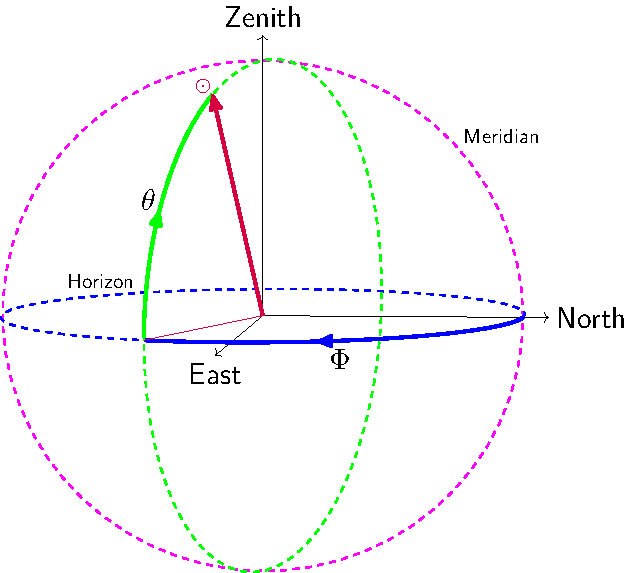
\includegraphics[scale=0.75]{horizontal-coordinate.pdf}
\caption{Horizontal coordinate system}
\label{fig:hz-coordinate}
\end{figure}

In this package, the cardinal points have specifics values of azimuth as following:

\begin{tabular}{c c c c}
North & East & South & West \\
0°    & 90°  & 180°  & 270°
\end{tabular}


The projection of the sun on the horizon plane is a point, which can be defined by two parameters:
\begin{itemize}
\item the angle $\Phi$,
\item the distance $r = \cos(\theta)$ from the centre to the sun.
\end{itemize}

Figure~\ref{fig:sun-projection} shows the projection of the sun on the horizontal plane.
If we track the position of sun on the horizontal plane changes from time to time, we will get a curve.
This curve is called the sun path. 
A chart which shows position of the sun from time to time is called a sun path chart.
Of course there are many type of sun path chart. 
This package provides tools to plot sun path on the horizontal plane.

\begin{figure}[H]
\centering
\begin{tikzpicture}[spradius=3]
\spcrosshair
\spaltitudecircle{{0}}
\spgeodirection[0pt]
\path[draw=red,fill=red](sunpath cs:azi=110,alt=66) circle[radius=2pt] ;
\end{tikzpicture}
\caption{Projection of the sun on the horizon plane}
\label{fig:sun-projection}
\end{figure}


\subsection{Draw a Sun path chart}

Figure~\ref{fig:sun-projection} is a very rudimentary sun path chart.
There is neither scalar, nor time on the chart. 
A more usable Sun path chart may look like one in the figure~\ref{fig:full-sun-path-chart}.
In this section we will create this chart.


\begin{figure}[H]
\centering
\begin{tikzpicture}
\spcrosshair
\spaltitudecircle{{0,10,...,80,85}}
\spazimuthline{{0,10,...,360}}{85}{70}
\spazimuthline{{0,5,...,360}}{80}{0}

\spazimuthtick

\spgeodirection
\spaltitudelabel{{10,20,...,80,85}}
\spazimuthlabel{{0,15,...,350}}

\path[draw=red,fill=red](sunpath cs:azi=110,alt=66) circle[radius=2pt] node[below] {{9:30}};
\end{tikzpicture}
\caption{A Sun path chart}
\label{fig:full-sun-path-chart}
\end{figure}

\subsubsection{Outlines}

User has to place \verb:\usepackage{sunpath}: in the preamble part of the document.

The chart is a \TikZ-picture, so we need a \texttt{tikzpicture}-environment.
We can also customize the distance from the centre of the chart to the horizon line by setup the option \texttt{spradius}.
By default it is 5.5 in PGF xy coordinate. 
In this example we make it a little bigger:

\marginpar{\texttt{spradius}}
\begin{verbatim}
\begin{tikzpicture}[spradius=6]
\end{tikzpicture}
\end{verbatim}

We also need the crosshair, the horizon line --in this type of sun path chart it is a circle--, 
the fours geographic direction.
This can be done by adding more commands into the \texttt{tikzpicture}

\begin{verbatim}
\begin{tikzpicture}[spradius=6]
\spcrosshair
\spaltitudecircle{{0}}
\spgeodirection
\end{tikzpicture}
\end{verbatim}

\marginpar{\texttt{drawcrosshair\\ drawgeodirection\\ drawaltitudecircle}}
\begin{tikzpicture}[spradius=6]
\spcrosshair
\spaltitudecircle{{0}}
\spgeodirection
\end{tikzpicture}


Man has to pay attention to the double curry brackets in the command \texttt{drawaltitudecircle}.
The outer brackets delimit the argument of the command.
The argument of the command is a valid \TikZ-range, which is used in a \verb:\foreach: command,
so it has be placed in between a pair of curry bracket. 
That is the inner brackets.


\subsubsection{Scalar and labels}


As the name of the commando says, we can also draw more than the horizon line by adding some values of altitude in the range of the argument of the command \verb|\spaltitudecircle|. 
For example \verb:\spaltitudecircle{{0,10,...,80,85}}: draws 10 circles of altitude.

\marginpar{\texttt{drawaltitudecircle}}
\begin{verbatim}
\begin{tikzpicture}[spradius=6]
\spcrosshair
\spaltitudecircle{{0,10,...,80,85}}
\spgeodirection
\end{tikzpicture}
\end{verbatim}

\begin{tikzpicture}[spradius=6]
\spcrosshair
\spaltitudecircle{{0,10,...,80,85}}
\spgeodirection
\end{tikzpicture}


We can use the command \verb:\drawazumuthline{r}{h}{l}: to draw azimuth lines in range \verb:r:, 
from the higher altitude \verb:h: to the lower altitude \verb:l:.

For example

\begin{itemize}
  \item \verb:\spazimuthline{{0,10,...,360}}{85}{70}: draws every 10° azimuth from the 85° altitude to to 70° altitude.
  \item \verb:\spazimuthline{{0,5,...,360}}{80}{0}: draws every 5° azimuth from the 80° altitude to to 0° altitude.
\end{itemize}

\begin{verbatim}
\begin{tikzpicture}[spradius=6]
\spcrosshair
\spaltitudecircle{{0,10,...,80,85}}
\spazimuthline{{0,10,...,360}}{85}{70}
\spazimuthline{{0,5,...,360}}{80}{0}

\spgeodirection
\end{tikzpicture}
\end{verbatim}

\marginpar{\texttt{drawazimuthline}}
\begin{tikzpicture}[spradius=6]
\spcrosshair
\spaltitudecircle{{0,10,...,80,85}}
\spazimuthline{{0,10,...,360}}{85}{70}
\spazimuthline{{0,5,...,360}}{80}{0}

\spgeodirection
\end{tikzpicture}

To draw azimuth ticks outside the horizon line, we can use 
\verb:\spazimuthtick:. 
This command expects for now no argument.

\begin{verbatim}
\begin{tikzpicture}[spradius=6]
\spcrosshair
\spaltitudecircle{{0,10,...,80,85}}
\spazimuthline{{0,10,...,360}}{85}{70}
\spazimuthline{{0,5,...,360}}{80}{0}
\spazimuthtick

\spgeodirection
\end{tikzpicture}
\end{verbatim}

\marginpar{\texttt{drawazimuthtick}}
\begin{tikzpicture}[spradius=6]
\spcrosshair
\spaltitudecircle{{0,10,...,80,85}}
\spazimuthline{{0,10,...,360}}{85}{70}
\spazimuthline{{0,5,...,360}}{80}{0}
\spazimuthtick

\spgeodirection
\end{tikzpicture}


To draw labels of azimuth lines and altitude circles in the chart, we can use the commands 

\verb:\spaltitudelabel{r}: and

\verb:\spazimuthlabel{r}:.

\begin{tikzpicture}[spradius=6]
\spcrosshair
\spaltitudecircle{{0,10,...,80,85}}
\spazimuthline{{0,10,...,360}}{85}{70}
\spazimuthline{{0,5,...,360}}{80}{0}
\spazimuthtick

\spaltitudelabel{{10,20,...,80,85}}
\spazimuthlabel{{0,15,...,350}}
\spgeodirection
\end{tikzpicture}

That it's, now we have a nice chart, on which we can draw positions of the sun from time to time.

\subsubsection{Position of the sun}

We can easily plot the position of the sun in the chart with the coordinate \texttt{sunpath}, 
if the azimuth and the altitude are given.
For example, to plot the position of the sun with 150° Azimuth and 22° Altitude, 
we just use the \texttt{path} command as following:

\verb|\path[fill=red,draw=red] (sunpath cs:azi=150,alt=22);|

The result would be

\begin{verbatim}
% ...
\path[fill=red,draw=red] (sunpath cs:azi=150,alt=35) circle[radius=2pt];
\spaltitudelabel{{10,20,...,80,85}}[160]
% ...
\end{verbatim}

\marginpar{\texttt{sunpath cs}}
\begin{tikzpicture}[spradius=6]
\spcrosshair
\spaltitudecircle{{0,10,...,80,85}}
\spazimuthline{{0,10,...,360}}{85}{70}
\spazimuthline{{0,5,...,360}}{80}{0}
\spazimuthtick

\path[fill=red,draw=red] (sunpath cs:azi=150,alt=35) circle[radius=2pt];

\spaltitudelabel{{10,20,...,80,85}}[160]
\spazimuthlabel{{0,15,...,350}}
\spgeodirection
\end{tikzpicture}

The command \verb:\spaltitudelabel: can also take an optional argument to set altitude label on other azimuth.
This can be useful if the labels cover distract important points on chart.
In this chart it is set to be 160°. So one can easily read the azimuth of the sun on the chart.

We can also connect the position of the sun to a path, for example with the positions given in the following table

{\ttfamily
\begin{tabular}{c  c  c}
Time  & Azimuth    & Altitude  \\
07:44 &  98.968673 & -0.208672 \\
08:00 & 102.009695 &  2.035492 \\
10:00 & 126.513583 & 19.499874 \\
12:00 & 156.854847 & 31.593335 \\
14:00 & 192.292832 & 33.425294 \\
16:00 & 224.708002 & 24.034984 \\
18:00 & 250.626597 &  7.619801 \\
18:53 & 260.810553 & -0.244637 \\
\end{tabular}
}

we can get a sun path like this:

\begin{tikzpicture}[spradius=6]
\tikzset{
  sunpath curve/.style={draw,fill=red},
  sunpath point/.style={radius=2pt,draw=red},
  sunpath node/.style={below,inner sep=0.5pt,outer sep=4.5pt,fill=white}
}
\spcrosshair
\spaltitudecircle{{0,10,...,80,85}}
\spazimuthline{{0,10,...,360}}{85}{70}
\spazimuthline{{0,5,...,360}}{80}{0}
\spazimuthtick

\path[sunpath curve] 
  (sunpath cs:azi=98.968673,alt=-0.208672) circle[sunpath point] node[sunpath node]{ { 07:44 } }
--(sunpath cs:azi=102.009695,alt=2.035492) circle[sunpath point] node[sunpath node]{ { 08:00 } }
--(sunpath cs:azi=126.513583,alt=19.499874) circle[sunpath point] node[sunpath node]{ { 10:00 } }
--(sunpath cs:azi=156.854847,alt=31.593335) circle[sunpath point] node[sunpath node]{ { 12:00 } }
--(sunpath cs:azi=192.292832,alt=33.425294) circle[sunpath point] node[sunpath node]{ { 14:00 } }
--(sunpath cs:azi=224.708002,alt=24.034984) circle[sunpath point] node[sunpath node]{ { 16:00 } }
--(sunpath cs:azi=250.626597,alt=7.619801) circle[sunpath point] node[sunpath node]{ { 18:00 } }
--(sunpath cs:azi=260.810553,alt=-0.244637) circle[sunpath point] node[sunpath node]{ { 18:53 } }
;

\spaltitudelabel{{10,20,...,80,85}}
\spazimuthlabel{{0,15,...,350}}
\spgeodirection
\end{tikzpicture}

But this chart is not nice. 
If the data is machine readable, we can generate all stuffs of the chart automatically.
This chart below is generated from the table above.
Just use your favourite programming language to process sun data.

\begin{tikzpicture}[spradius=6]
\tikzset{
  sun path curve/.style={draw=red!20,thick},
  sun point/.style={radius=2pt,draw=red,fill=red},  
  sun label/.style={below,fill=white,outer sep=4pt,text=red},
}
\spcrosshair
\spaltitudecircle{{0,10,...,80,85}}
\spazimuthline{{0,10,...,360}}{85}{70}
\spazimuthline{{0,5,...,360}}{80}{0}
\spazimuthtick

\coordinate (P0) at (sunpath cs:azi=98.968673,alt=-0.208672);
\coordinate (P1) at (sunpath cs:azi=102.009695,alt=2.035492);
\coordinate (P2) at (sunpath cs:azi=126.513583,alt=19.499874);
\coordinate (P3) at (sunpath cs:azi=156.854847,alt=31.593335);
\coordinate (P4) at (sunpath cs:azi=192.292832,alt=33.425294);
\coordinate (P5) at (sunpath cs:azi=224.708002,alt=24.034984);
\coordinate (P6) at (sunpath cs:azi=250.626597,alt=7.619801);
\coordinate (P7) at (sunpath cs:azi=260.810553,alt=-0.244637);
\path[sun point] (P0) circle;
\path[sun point] (P1) circle;
\path[sun point] (P2) circle;
\path[sun point] (P3) circle;
\path[sun point] (P4) circle;
\path[sun point] (P5) circle;
\path[sun point] (P6) circle;
\path[sun point] (P7) circle;
\node[sun label,anchor=270-98.968673] at (P0) {07:44};
\node[sun label,anchor=270-102.009695] at (P1) {08:00};
\node[sun label,anchor=270-126.513583] at (P2) {10:00};
\node[sun label,anchor=270-156.854847] at (P3) {12:00};
\node[sun label,anchor=270-192.292832] at (P4) {14:00};
\node[sun label,anchor=270-224.708002] at (P5) {16:00};
\node[sun label,anchor=270-250.626597] at (P6) {18:00};
\node[sun label,anchor=270-260.810553] at (P7) {18:53};
\path[sun path curve] (P0) to [curve through={ (P1) .. (P2) .. (P3) .. (P4) .. (P5) .. (P6) }] (P7) ;

\spaltitudelabel{{10,20,...,80,85}}[170]
\spazimuthlabel{{0,15,...,350}}
\spgeodirection
\end{tikzpicture}

\vfill\newpage
The part, which makes the chart nicer, is there:

\begin{verbatim}
%...
\coordinate (P0) at (sunpath cs:azi=98.968673,alt=-0.208672);
\coordinate (P1) at (sunpath cs:azi=102.009695,alt=2.035492);
\coordinate (P2) at (sunpath cs:azi=126.513583,alt=19.499874);
\coordinate (P3) at (sunpath cs:azi=156.854847,alt=31.593335);
\coordinate (P4) at (sunpath cs:azi=192.292832,alt=33.425294);
\coordinate (P5) at (sunpath cs:azi=224.708002,alt=24.034984);
\coordinate (P6) at (sunpath cs:azi=250.626597,alt=7.619801);
\coordinate (P7) at (sunpath cs:azi=260.810553,alt=-0.244637);
\path[sun point] (P0) circle;
\path[sun point] (P1) circle;
\path[sun point] (P2) circle;
\path[sun point] (P3) circle;
\path[sun point] (P4) circle;
\path[sun point] (P5) circle;
\path[sun point] (P6) circle;
\path[sun point] (P7) circle;
\node[sun label,anchor=270-98.968673] at (P0) {07:44};
\node[sun label,anchor=270-102.009695] at (P1) {08:00};
\node[sun label,anchor=270-126.513583] at (P2) {10:00};
\node[sun label,anchor=270-156.854847] at (P3) {12:00};
\node[sun label,anchor=270-192.292832] at (P4) {14:00};
\node[sun label,anchor=270-224.708002] at (P5) {16:00};
\node[sun label,anchor=270-250.626597] at (P6) {18:00};
\node[sun label,anchor=270-260.810553] at (P7) {18:53};
\path[sun path curve] (P0) to [curve through={ 
    (P1) .. (P2) .. (P3) .. (P4) .. (P5) .. (P6) 
    }] 
  (P7) ;
%...
\end{verbatim}

To set the altitude scale (and also the altitude lines) equidistance, just use the option \verb|altitude mapping=equidistance|.
The chart above with same data looks like the chart below with this option.

\marginpar{\texttt{altitude mapping}} \texttt{ = equidistance}

\begin{tikzpicture}[spradius=6,altitude mapping=equidistance]
\tikzset{
  sun path curve/.style={draw=red!20,thick},
  sun point/.style={radius=2pt,draw=red,fill=red},  
  sun label/.style={below,fill=white,outer sep=4pt,text=red},
}
\spcrosshair
\spaltitudecircle{{0,10,...,80,85}}
\spazimuthline{{0,10,...,360}}{85}{70}
\spazimuthline{{0,5,...,360}}{80}{0}
\spazimuthtick

\coordinate (P0) at (sunpath cs:azi=98.968673,alt=-0.208672);
\coordinate (P1) at (sunpath cs:azi=102.009695,alt=2.035492);
\coordinate (P2) at (sunpath cs:azi=126.513583,alt=19.499874);
\coordinate (P3) at (sunpath cs:azi=156.854847,alt=31.593335);
\coordinate (P4) at (sunpath cs:azi=192.292832,alt=33.425294);
\coordinate (P5) at (sunpath cs:azi=224.708002,alt=24.034984);
\coordinate (P6) at (sunpath cs:azi=250.626597,alt=7.619801);
\coordinate (P7) at (sunpath cs:azi=260.810553,alt=-0.244637);
\path[sun point] (P0) circle;
\path[sun point] (P1) circle;
\path[sun point] (P2) circle;
\path[sun point] (P3) circle;
\path[sun point] (P4) circle;
\path[sun point] (P5) circle;
\path[sun point] (P6) circle;
\path[sun point] (P7) circle;
\node[sun label,anchor=270-98.968673] at (P0) {07:44};
\node[sun label,anchor=270-102.009695] at (P1) {08:00};
\node[sun label,anchor=270-126.513583] at (P2) {10:00};
\node[sun label,anchor=270-156.854847] at (P3) {12:00};
\node[sun label,anchor=270-192.292832] at (P4) {14:00};
\node[sun label,anchor=270-224.708002] at (P5) {16:00};
\node[sun label,anchor=270-250.626597] at (P6) {18:00};
\node[sun label,anchor=270-260.810553] at (P7) {18:53};
\path[sun path curve] (P0) to [curve through={ (P1) .. (P2) .. (P3) .. (P4) .. (P5) .. (P6) }] (P7) ;

\spaltitudelabel{{10,20,...,80,85}}[170]
\spazimuthlabel{{0,15,...,350}}
\spgeodirection
\end{tikzpicture}




\vfill\newpage
% get the document about implementation inside main document
\DocInput{\jobname.dtx}

\PrintChanges
\PrintIndex
\end{document}
